% ---- title metadata --------------------------------------------------------
\title{Growth \& Remodeling of Soft Tissue}
\subtitle{A hands-on introduction to the four modelling frameworks}
\author{}
\date{}

\begin{document}

% ---- title frame -----------------------------------------------------------
{%
\setbeamertemplate{footline}{}
\begin{frame}[plain]
  \vfill
  \begin{center}
    {\Large\bfseries\color{YaleBlue} Growth \& Remodeling of Soft Tissue}\\[0.6em]
    {\color{BoxGray} A hands-on introduction to the four modelling frameworks}\\[1.4em]
    {\small kinematic growth $\;\cdot\;$ constrained mixture $\;\cdot\;$ homogenized $\;\cdot\;$ equilibrated}\\[2.2em]
    \ifteacher
      {\footnotesize\color{AccentRed} teacher version --- key equations filled in}
    \else
      {\footnotesize\color{YaleLightBlue} student version --- boxes to fill in during class}
    \fi
  \end{center}
  \vfill
  {\scriptsize\color{BoxGray} Reproducible figures generated by the \texttt{gr} package \textendash\ \texttt{github.com/YaleCBL-Teaching/Growth-Remodeling}}
\end{frame}
}

% ---- section files ---------------------------------------------------------
% ============================================================================
%  SECTION 1 — Biological motivation & fundamental observations
%  Order: motivation plots first; constituents introduced only at the end.
% ============================================================================
\begin{frame}[t]{}
  \vfill\begin{center}{\Huge\color{YaleBlue} The biology}
  \end{center}\vfill
\end{frame}

\begin{frame}[t]{Living Materials Are Never ``Finished''}
  A steel beam is made once and wears out. A living artery is
  \textbf{continuously torn down and rebuilt}: cells deposit and degrade
  structural proteins while sensing the loads they carry.
  \begin{itemize}
    \item \textbf{Growth} --- change in \emph{mass}.
    \item \textbf{Remodeling} --- change in \emph{microstructure} (fiber
    orientation, natural length, composition).
  \end{itemize}
  \vfill
  \begin{center}\color{AccentRed}
  Will a hypertensive artery thicken and stabilise, or an aneurysm dilate to
  rupture?
  \end{center}
\end{frame}

\begin{frame}[t]{Cells Actively Hold a Mechanical Set-Point}
  Cultured cells generate a steady \textbf{tension} and \emph{restore} it after
  each perturbation --- direct evidence that living tissue targets a mechanical
  state rather than a fixed shape.
  \bigfigw{biol_tensional_homeostasis.png}{0.72\linewidth}{Force generated by a
  contractile cell line vs.\ control, recovering after repeated unloading.}
  \srccite{Tensional homeostasis; Brown et al., J Cell Physiol (1998)}
\end{frame}

\begin{frame}[t]{Fundamental Observation: A Stress Set-Point}
  Wolinsky \& Glagov (1967): Cauchy stress in the aortic media is nearly
  \textbf{constant across mammals} spanning orders of magnitude in body mass ---
  tissue-level evidence of a mechanical set-point.
  \bigfigw{motiv_wolinsky_glagov.png}{0.6\linewidth}{Wall tension vs.\ body mass
  across species.}
  \srccite{Wolinsky \& Glagov, Circ Res (1967)}
\end{frame}

\begin{frame}[t]{Cells Chase a Mechanical Set-Point}
  Cells regulate a \textbf{target (homeostatic) stress}: above it they build more,
  below it removal wins --- a negative feedback that thickens a hypertensive wall
  until stress returns to normal.
  \vfill
  \begin{center}\gnrloop[0.86]\end{center}
  \vfill
  \srccite{Humphrey, J Elasticity (2021)}
\end{frame}

\begin{frame}[t]{Two Canonical Scenarios We Will Simulate}
  \begin{columns}[T]
    \begin{column}{0.5\textwidth}
      \textbf{\color{YaleBlue}Hypertension} --- sustained pressure step. Expect
      \emph{adaptation}: the wall thickens, stress returns to set-point.
    \end{column}
    \begin{column}{0.5\textwidth}
      \textbf{\color{YaleBlue}Aneurysm} --- irreversible elastin loss. Geometry can
      feed \emph{positively} back on stress: stabilise larger, \emph{or} dilate
      without bound.
    \end{column}
  \end{columns}
  \vfill
  \begin{center}\large\color{AccentRed}
  \emph{When does a tissue adapt, and when does it run away?}
  \end{center}
\end{frame}

% ---- constituents introduced only at the END of the biology section --------
\begin{frame}[t]{The Cast of Characters in an Arterial Wall}
  \footnotesize
  \begin{center}
  \renewcommand{\arraystretch}{1.35}
  \begin{tabular}{@{}p{0.135\textwidth}p{0.235\textwidth}p{0.115\textwidth}p{0.115\textwidth}p{0.30\textwidth}@{}}
    \toprule
    \textbf{Constituent} & \textbf{Mechanical role} & \textbf{Mass frac.\ $\phi$} &
      \textbf{Dep.\ stretch $G$} & \textbf{Material model \& turnover $1/k_d$}\\
    \midrule
    \textbf{\color{YaleBlue}Elastin} & soft; bears load at low stretch & $0.30$ & $1.40$ &
      neo-Hookean ($c\approx90$\,kPa); \textbf{none} (decades) \\
    \textbf{\color{YaleBlue}Collagen} & stiff, crimped; guards against rupture & $0.35$ & $1.08$ &
      Fung ($c_1\approx250$\,kPa, $c_2\approx8$); \textbf{fast} ($\sim$20\,d) \\
    \textbf{\color{YaleBlue}Smooth muscle} & passive load + active contraction; the sensor cell &
      $0.35$ & $1.20$ & Fung ($c_1\approx120$\,kPa, $c_2\approx3$); fast ($\sim$20\,d) \\
    \bottomrule
  \end{tabular}
  \end{center}
  \vfill
  \begin{itemize}\footnotesize
    \item \textbf{Elastin cannot be renewed} --- its loss triggers \emph{aneurysm}.
    \item \textbf{Collagen \& SMC turn over constantly} --- so the wall can
    \emph{adapt}, or \emph{run away}.
  \end{itemize}
  \begin{center}\scriptsize\color{BoxGray}
  Teaching-grade values for a large elastic artery, in the range used by Humphrey,
  Cyron, Latorre and co-workers (order-of-magnitude, not a fit to one animal).
  \end{center}
  \srccite{Humphrey, Eberth, Dye, Gleason, J Biomech (2009)}
\end{frame}

% ============================================================================
%  SECTION 1b — Mechanical stimuli: Laplace law & wall shear stress (EARLY)
% ============================================================================
\begin{frame}[t]{An Idealized Blood Vessel}
  A vessel is a \textbf{pressurised, perfused tube}. Two loads act on the wall:
  \textbf{blood pressure} $P$ pushes it outward, and \textbf{blood flow} $Q$ drags
  its inner surface. Cells sense both.
  \vfill
  \begin{center}\idealvessel[0.60]\end{center}
  \vfill
  \begin{center}\small
  $P$ lumen pressure $\to$ \textbf{circumferential stress} $\sigma_\theta$
  \qquad
  $Q$ volumetric flow $\to$ \textbf{wall shear stress} $\tau_w$
  \qquad
  $a$ inner radius, \ $h$ wall thickness
  \end{center}
  \srccite{Humphrey, Cardiovascular Solid Mechanics (2002)}
\end{frame}

\begin{frame}[t]{Two Loads, Two Formulae, Two Adaptations}
  Pressure $P$ sets the \textbf{hoop stress}; flow $Q$ sets the \textbf{wall shear
  stress}. Each has a set-point; rearranging shows the geometry that restores it.
  \vfill
  \begin{columns}[T]
    \begin{column}{0.5\textwidth}
      \begin{center}\textbf{\color{YaleBlue} Pressure} (Laplace)\end{center}
      \slboxeq{2.4em}{eq:laplace}{\sigma_\theta = P\,\frac{a}{h}}
      Hold $\sigma_\theta=\sigma_{\theta,h}$: $\;h=Pa/\sigma_{\theta,h}\propto P$
      --- higher pressure $\Rightarrow$ \textbf{thicker wall}.
    \end{column}
    \begin{column}{0.5\textwidth}
      \begin{center}\textbf{\color{YaleBlue} Flow} (Poiseuille)\end{center}
      \slboxeq{2.4em}{eq:wss}{\tau_w = Q\,\frac{4\mu}{\pi\,a^3}}
      Hold $\tau_w=\tau_{w,h}$: $\;a=(4\mu Q/\pi\tau_{w,h})^{1/3}\propto Q^{1/3}$
      --- higher flow $\Rightarrow$ \textbf{larger lumen}.
    \end{column}
  \end{columns}
  \vfill
  \srccite{Laplace \& Poiseuille; Humphrey, Cardiovascular Solid Mechanics (2002)}
\end{frame}

% ---- interactive analytical exercises (pen & paper) ------------------------
\begin{frame}[t]{}
  \begin{yourturnbox}{Pressure adaptation}
    \qq{Pressure \textbf{doubles} ($P'=2P$), radius $a$ fixed. By how much must the
    wall thicken to restore $\sigma_{\theta,h}$?}
    \qhint{Set $P'a/h'=\sigma_{\theta,h}=Pa/h$; solve for $h'$.}
  \end{yourturnbox}
\end{frame}

\begin{frame}[t]{}
  \begin{answerbox}{Pressure adaptation}
    $P'a/h'=Pa/h$ with $P'=2P$ gives
    \slboxeq{2.2em}{eq:ans:pressure}{h' = 2\,h.}
    \par\smallskip
    {\color{ABlue}\bfseries Reading.} Wall thickens \emph{in proportion} to
    pressure (Grossman) --- radius unchanged, stress restored.
  \end{answerbox}
  \srccite{Grossman, Jones, McLaurin, J Clin Invest (1975)}
\end{frame}

\begin{frame}[t]{}
  \begin{yourturnbox}{Flow adaptation}
    \qq{Flow rises \textbf{8-fold} ($Q'=8Q$). By how much must the radius change to
    restore $\tau_{w,h}$?}
    \qhint{$\tau_w\propto Q/a^3$; set $\tau_w(Q',a')=\tau_{w,h}$ and solve for $a'$.}
  \end{yourturnbox}
\end{frame}

\begin{frame}[t]{}
  \begin{answerbox}{Flow adaptation}
    $(a'/a)^3 = Q'/Q = 8$, so
    \slboxeq{2.2em}{eq:ans:flow}{a' = 8^{1/3}\,a = 2\,a.}
    \par\smallskip
    {\color{ABlue}\bfseries Reading.} Radius grows as the \emph{cube root} of flow
    --- flow-induced outward remodeling; an 8$\times$ flow only doubles the lumen.
  \end{answerbox}
  \srccite{Kamiya \& Togawa, Am J Physiol (1980)}
\end{frame}

% ============================================================================
%  SECTION 2 — Mathematical details / finite-strain fundamentals
% ============================================================================
\begin{frame}[t]{}
  \vfill\begin{center}{\Huge\color{YaleBlue} 2.\ \ Finite-strain fundamentals}\\[0.5em]
  {\color{BoxGray} just enough continuum mechanics to read the four theories}\end{center}\vfill
\end{frame}

\begin{frame}[t]{Deformation, stretch, and (in)compressibility}
  A body deforms from a \textbf{reference} to a \textbf{current} configuration; the
  deformation gradient $\bm{F}$ maps reference line elements to current ones.
  Everything here collapses to one dominant direction (bar axis, or artery
  circumference), so we track a single scalar \textbf{stretch}
  \giveneq{\lambda = \frac{\text{current length}}{\text{reference length}},\qquad
    \lambda=1\ \text{undeformed},\quad \lambda>1\ \text{extension}.}
  The tissue is \textbf{elastically incompressible} --- only \emph{growth} changes
  volume --- so the through-thickness and transverse stretches follow from
  $\lambda$ alone. One number suffices.
  \vspace{0.4em}

  We report the \textbf{Cauchy (true) stress} $\sigma$ (force per unit
  \emph{current} area): the physically meaningful measure for a growing body,
  because the load-bearing area itself changes as the tissue remodels.
  \srccite{finite-strain background adapted from YaleCBL-Teaching/BENG\_5570}
\end{frame}

\begin{frame}[t]{Wall stress from the loading --- the Laplace law}
  For a pressurised thin tube (the artery), the circumferential wall stress is
  \slboxeq{2.6em}{eq:laplace}{\sigma_\theta = \frac{P\,r}{h}}
  with pressure $P$, current inner radius $r$, wall thickness $h$. The bar instead
  carries a stress set by an \emph{axial} load. The consequence, drawn out on the
  right: the ``required stress'' the loading demands grows
  \textbf{linearly} in $\lambda$ for the bar, but \textbf{quadratically} for the
  artery.
  \vspace{0.3em}
  \begin{columns}[T]
    \begin{column}{0.46\textwidth}
      \begin{itemize}\small
        \item bar: $\ \sigma_{\text{req}}\propto \lambda^1 / (M/M_0)$
        \item artery: $\ \sigma_{\text{req}}\propto \lambda^2 / (M/M_0)$
      \end{itemize}
      {\color{AccentRed}\small That extra power of $\lambda$ is the whole story of
      arterial instability (§7).}
    \end{column}
    \begin{column}{0.54\textwidth}
      \vspace{-0.6em}\slidefig[\linewidth]{fig01_constitutive.pdf}
    \end{column}
  \end{columns}
  \figcredit{Right panel reproduced with the \texttt{gr} package (this repo)}
\end{frame}

\begin{frame}[t]{Hyperelastic constituents}
  Each constituent stores energy in a strain-energy function; its stress is the
  derivative. We use the two laws that describe arterial tissue.
  \vspace{0.3em}

  \textbf{Elastin --- neo-Hookean} (soft, barely stiffening):
  \giveneq{\sigma_e(\lambda_e) = c_e\!\left(\lambda_e^2 - \tfrac{1}{\lambda_e}\right).}

  \textbf{Collagen \& smooth muscle --- Fung exponential fiber} (crimped, then
  stiffens steeply once recruited):
  \slboxeq{2.8em}{eq:fung}{\sigma(\lambda_e) = c_1\,\lambda_e^2\,(\lambda_e^2-1)\,
    e^{\,c_2(\lambda_e^2-1)^2},\qquad I_4=\lambda_e^2}
  These are exactly the constituent free energies used in the constrained-mixture
  literature. The tangent $\dd\sigma/\dd\lambda_e$ is also needed --- for
  equilibrium solves and for the stability analysis (§7).
  \srccite{constituent laws as in Latorre, Humphrey, Comput Methods Appl Mech Eng (2020)}
\end{frame}

\begin{frame}[t]{The deposition stretch $G^k$ --- the crucial modelling idea}
  Cells deposit new fibers \textbf{already under tension}, at a fixed
  \textbf{deposition stretch} $G^k>1$. So at homeostasis a constituent's elastic
  stretch equals its own $G^k$, and we \emph{define} its homeostatic stress from
  that set-point:
  \slboxeq{2.4em}{eq:setpoint}{\sigma_h^k := \sigma^k(G^k)}
  This single convention pins down \emph{every} set-point in the course from a few
  physical inputs --- and is why all four theories can share one parameter set and
  give apples-to-apples comparisons.
  \srccite{deposition-stretch concept: Humphrey, Rajagopal, Math Models Methods Appl Sci (2002)}
\end{frame}

\begin{frame}[t]{Multiplicative decomposition --- growth vs.\ elasticity}
  The single most important kinematic idea in G\&R: split the deformation into a
  stress-free \textbf{inelastic} part (growth / remodeling) and an \textbf{elastic}
  part --- the only part that carries stress. In 1D,
  \slboxeq{2.4em}{eq:split}{\lambda = \lambda_e \,\lambda_{\text{inel}}}
  \begin{itemize}
    \item \textbf{Kinematic growth} (§3) uses \emph{one} such split with an
    inelastic \emph{growth} stretch.
    \item \textbf{Constrained mixtures} (§4) give \emph{each cohort of each
    constituent} its own inelastic natural configuration, and superpose them.
  \end{itemize}
  \vspace{0.4em}
  The set-point \eqref{eq:setpoint} and the split \eqref{eq:split} are the two
  pieces of machinery reused in every model that follows.
\end{frame}

% ============================================================================
%  SECTION 3 — Kinematic growth
% ============================================================================
\begin{frame}[t]{}
  \vfill\begin{center}{\Huge\color{YaleBlue} 3.\ \ Kinematic growth}\\[0.5em]
  {\color{BoxGray} Rodriguez, Hoger \& McCulloch (1994)}\end{center}\vfill
\end{frame}

\begin{frame}[t]{The idea, and the kinematics}
  Postulate a stress-free \textbf{growth} deformation; only the elastic part
  carries load. Growth is one scalar $\theta$ (radial thickening):
  \giveneq{\bm{F} = \bm{F}_e\,\bm{F}_g,\qquad \frac{M}{M_0}=\theta,\qquad
    \text{only }\bm{F}_e\text{ stores energy.}}
  \bigfigw{kin_multiplicative_split.png}{0.62\linewidth}{One growth variable for
  the whole mixture --- no individual turnover. That is the strength and the
  ceiling.}
  \figcredit{Fig.: A. Gebauer (TUM lecture); Rodriguez, Hoger, McCulloch, J Biomech (1994)}
\end{frame}

\begin{frame}[t]{The growth law}
  Growth nulls the stress deviation from the set-point (first-order, production
  $\propto$ current mass):
  \slboxeq{2.6em}{eq:kingrowth}{\frac{\dd\theta}{\dd t}
    = k_g\,\theta\left(\frac{\bar\sigma}{\bar\sigma_h}-1\right)}
  The set-point $\bar\sigma_h$ is \textbf{prescribed}: wherever growth stops
  ($\dot\theta=0$), stress is homeostatic \emph{by construction}. At each instant
  $\lambda$ follows from equilibrium
  $\bar\sigma(\lambda)=\sigma_{\text{req}}(\lambda,\theta)$.
  \srccite{Rodriguez, Hoger, McCulloch, J Biomech (1994)}
\end{frame}

\begin{frame}[t]{Stability is imposed, not predicted}
  Growth is stable iff adding mass \emph{lowers} the stress it must carry,
  $\left.\dd\bar\sigma/\dd\theta\right|_{\theta^*}<0$ --- always true for the
  \textbf{bar}, but a strong enough insult flips the sign for the \textbf{artery}
  (Laplace $\lambda^2$) and growth runs away.
  \bigfigw{fig02_kinematic_growth.pdf}{0.78\linewidth}{Kinematic growth either
  converges to the \emph{prescribed} set-point or diverges --- it cannot
  \emph{predict} stability from turnover.}
  \figcredit{Reproduced with the \texttt{gr} package (this repo)}
\end{frame}

\begin{frame}[t]{}
  \vfill\begin{center}{\Huge\color{YaleBlue} The Constrained Mixture Model}
  \end{center}\vfill
\end{frame}

\begin{frame}[t]{One Framework, Many Applications}
  \vfill
  \begin{center}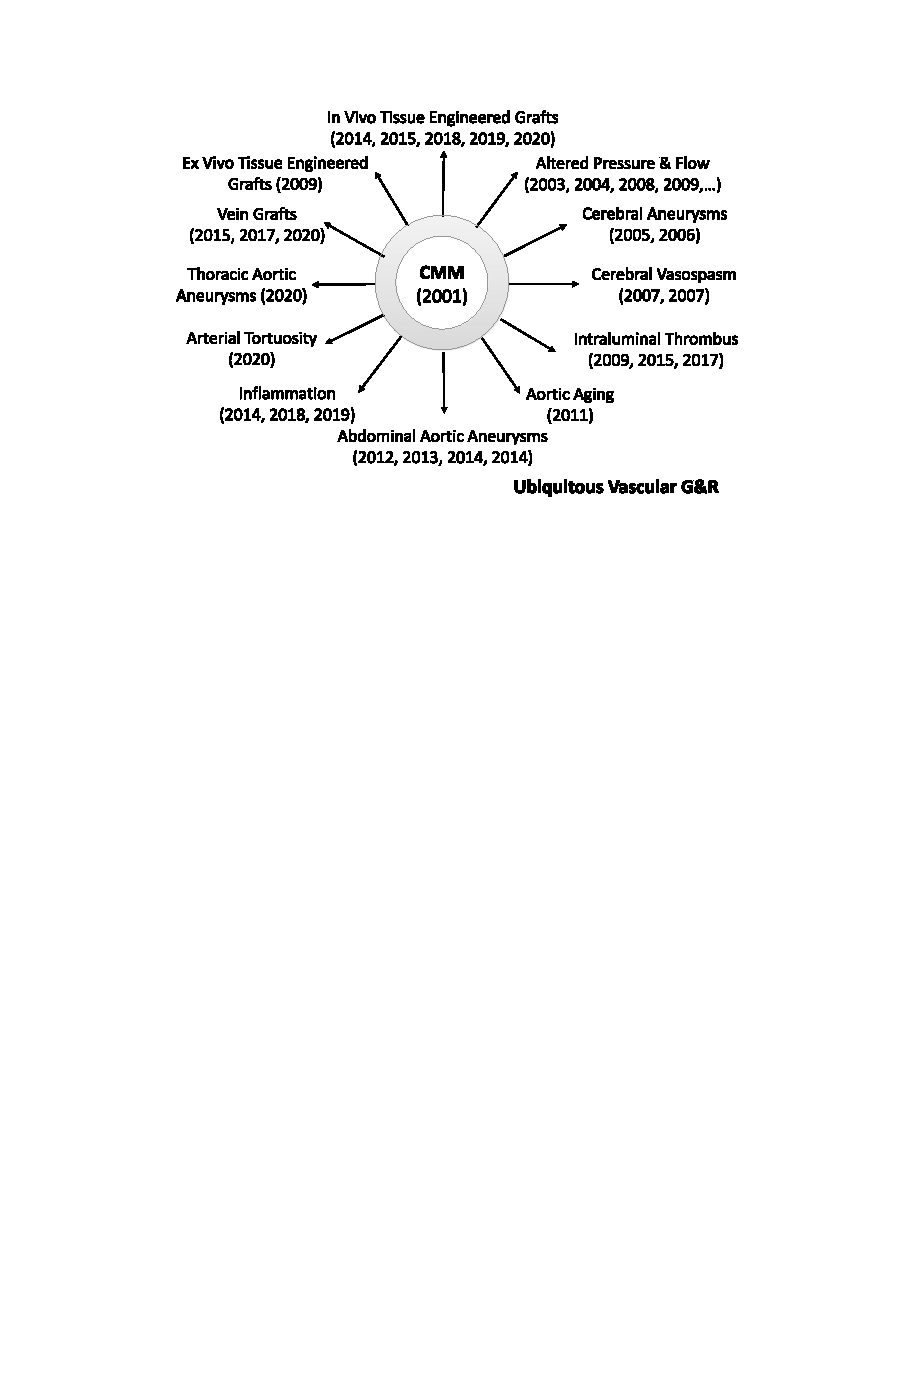
\includegraphics[height=0.9\textheight]{figures/cmm_applications.pdf}\end{center}
  \vfill
  \srccite{Humphrey, J Elasticity (2021)}
\end{frame}

\begin{frame}[t]{The Idea: Track Every Cohort}
  \vfill
  \begin{center}\humphreygr[0.56]\end{center}
  \vspace{-0.1em}
  \begin{center}\footnotesize\color{black!70}
  $\kappa$: configuration \;\textbullet\; $\tau$: deposition time \;\textbullet\;
  $s$: current time \;\textbullet\; $\alpha$: constituent
  \;\textbullet\; $\bm{G}^{\alpha}$: deposition stretch \;\textbullet\;
  $\bm{F}^{\alpha}_{n(\tau)}$: constituent deformation
  \end{center}
  \vfill
  \srccite{Humphrey, J Elasticity (2021)}
\end{frame}

\begin{frame}[t]{Load-Bearing Vessel Constituents}
  \footnotesize
  The wall is a mixture of three constituents, each with a reference \textbf{mass
  fraction} $\phi_0^{\alpha}$ ($\sum_\alpha\phi_0^{\alpha}=1$) and a
  \textbf{deposition stretch} $G^{\alpha}$ --- the prestretch cells lay it down at,
  which \emph{defines} its homeostatic stress
  $\sigma_h^{\alpha}=\sigma^{\alpha}(G^{\alpha})$; the mixture set-point is
  $\bar\sigma_h=\sum_\alpha\phi_0^{\alpha}\sigma_h^{\alpha}$.
  \vspace{0.3em}
  \renewcommand{\arraystretch}{1.3}
  \begin{center}
  \begin{tabular}{@{}p{0.15\textwidth}p{0.28\textwidth}ccp{0.24\textwidth}@{}}
    \toprule
    \textbf{Constituent} & \textbf{Role} & $\phi_0$ & $G^{\alpha}$ & \textbf{law; turnover $1/k_d$}\\
    \midrule
    \textbf{\color{YaleBlue}Elastin} & bears load at low stretch & 0.30 & 1.40 &
      neo-Hooke; \textbf{none} (decades)\\
    \textbf{\color{YaleBlue}Collagen} & stiff, crimped; anti-rupture & 0.35 & 1.08 &
      Fung; fast ($\sim$20\,d)\\
    \textbf{\color{YaleBlue}Smooth muscle} & passive + active; the sensor & 0.35 & 1.20 &
      Fung; fast ($\sim$20\,d)\\
    \bottomrule
  \end{tabular}
  \end{center}
  \vspace{0.3em}
  \textbf{Elastin cannot be renewed} ($k_d^e=0$) --- its loss drives
  \emph{aneurysm}; collagen \& SMC \textbf{turn over}, so the wall can
  \emph{adapt}.
  \srccite{Humphrey, Eberth, Dye, Gleason, J Biomech (2009)}
\end{frame}

\begin{frame}[t]{Every Cohort Shares One Stretch}
  A cohort of $\alpha$ deposited at $\tau$ is laid down at $G^{\alpha}$ and then
  stretches \emph{with the mixture}: every constituent and cohort is
  \textbf{constrained} to the same tissue stretch $\lambda(s)$.
  \dlab{constituent-specific deformation}
  \giveneq{\bm{F}^{\alpha}_{n(\tau)}(s) = \bm{F}(s)\,\bm{F}^{-1}(\tau)\,\bm{G}^{\alpha}(\tau).}
  \zlab{scalar elastic stretch}
  \slboxeq{eq:cohort}{\lambda_{n(\tau)}^{\alpha}(s,\tau) = \frac{\lambda(s)}{\lambda(\tau)} \, G^{\alpha}}
  \srccite{Humphrey, Rajagopal, Math Models Methods Appl Sci (2002)}
\end{frame}

% ---- derivation after Humphrey (2021): mass balance (1) ----------------------
\begin{frame}[t]{Mass Balance}
  Track each constituent's
  \textbf{apparent mass density} $\rho^{\alpha}$ per current
  mixture volume, $\rho=\sum_{\alpha}\rho^{\alpha}$.
  \par\medskip
  Spatial mass balance (one per constituent):
  \giveneq{\frac{\partial\rho^{\alpha}}{\partial s}
     + \underbrace{\operatorname{div}(\rho^{\alpha}\bm{v}^{\alpha})}_{\text{transport}}
     = \underbrace{\bar m^{\alpha}}_{\text{net mass exchange}},
     \qquad \alpha=1,\dots,N.}
  The net rate is \emph{signed}:
  \giveneq{\bar m^{\alpha}=\underbrace{m^{\alpha}}_{\text{production}\ge 0}
     -\underbrace{r^{\alpha}}_{\text{removal}\ge 0}
     \;\begin{cases}
       <0 & \text{atrophy}\\[2pt]
       =0 & \text{maintenance}\\[2pt]
       >0 & \text{growth}
     \end{cases}}
  \srccite{Humphrey, J Elasticity (2021)}
\end{frame}

% ---- assumptions 1 & 2 -> heredity integral (2) ------------------------------
\begin{frame}[t]{From Balance to a Heredity Integral}
  \textbf{Assumption 1 (constrained mixture):} every constituent moves with the
  mixture, $\bm{v}^{\alpha}=\bm{v}$.
  \par\smallskip
  \textbf{Assumption 2 (prescribed rates):} a true production rate
  $m^{\alpha}(\tau)\ge 0$ and a survival fraction $q^{\alpha}(s,\tau)\in[0,1]$.
  Integrating from the distant past to $s$:
  \slboxeq{eq:massher}{\rho^{\alpha}(s)=
     \underbrace{\rho^{\alpha}(0)\,Q^{\alpha}(s)}_{\text{survivors of original material}}
     +\underbrace{\int_{0}^{s} m^{\alpha}(\tau)\,q^{\alpha}(s,\tau)\,\dd\tau}
       _{\text{deposited at }\tau,\ \text{still present at }s}}
  with $Q^{\alpha}(0)=1$. \textbf{Assumption 3:} bulk density is nearly constant,
  $\rho(s)=\rho(0)$ --- mass changes track volume changes.
  \srccite{Humphrey, J Elasticity (2021)}
\end{frame}

\begin{frame}[t]{Linear Momentum Balance}
  A rule-of-mixtures for the stresses (no body forces) satisfies the classical
  linear-momentum balance:
  \giveneq{\operatorname{div}\bm{\sigma}=\rho\,\bm{a}
     \;\;\xrightarrow{\ \text{quasi-static}\ }\;\;
     \operatorname{div}\bm{\sigma}=\bm{0}.}
  \textbf{Quasi-static assumption:} G\&R evolves slowly at every time $s$, so the
  inertia $\rho\bm{a}$ is negligible.
  \srccite{Humphrey, J Elasticity (2021)}
\end{frame}

\begin{frame}[t]{Constitutive Relations: Cauchy Stress}
  In finite elasticity the Cauchy stress follows from a stored-energy function
  $W$ (per unit reference mixture volume):
  \giveneq{\bm{\sigma}(s)=\frac{2}{J}\,\bm{F}(s)\,
     \frac{\partial W(s)}{\partial\bm{C}(s)}\,\bm{F}^{\mathrm{T}}(s),
     \qquad \bm{C}=\bm{F}^{\mathrm{T}}\bm{F},\quad J=\det\bm{F}.}
  Rule of mixtures: $W=\sum_{\alpha}\tilde W^{\alpha}$. Closing the model needs
  \textbf{three constituent-specific relations} --- a \emph{stored energy}
  $W^{\alpha}$, a \emph{production} rate $m^{\alpha}$, and a \emph{removal}
  (survival) $q^{\alpha}$.
  \srccite{Humphrey, J Elasticity (2021)}
\end{frame}

\begin{frame}[t]{Three Constituent-Specific Constitutive Relations}
  \textbf{1.\ Material:} constituent stored energy $W^{\alpha}$: neo-Hookean
  elastin, Fung-type collagen \& smooth muscle (eq.~\eqref{eq:fung}).
  \par\medskip
  \textbf{2.\ Rate of production:} up with wall stress \& inflammation, down
  with wall shear:
  \slboxeq{eq:production}{m^{\alpha}(\tau)=m_o^{\alpha}\big(1
     + K_{\sigma}^{\alpha}\,\Delta\sigma
     - K_{\tau_w}^{\alpha}\,\Delta\tau_w
     + K_{\varphi}^{\alpha}\,\Delta\rho_{\varphi}\big)\ge 0}
  \vspace{-0.4em}
  \begin{center}\footnotesize\color{black!70}
   $\Delta\sigma$: pressure \;\textbullet\; $\Delta\tau_w$: flow \;\textbullet\;
   $\Delta\rho_{\varphi}$: inflammation
  \end{center}
  \textbf{3.\ Rate of removal:} a survival fraction that decays faster under
  stress perturbation:
  \slboxeq{eq:removal}{q^{\alpha}(s,\tau)=\exp\!\Big(\!-\!\int_{\tau}^{s}
     k_o^{\alpha}\big(1+\omega\,\Delta\sigma^{2}(t)+\cdots\big)\,\dd t\Big)\in[0,1]}
  \srccite{Valentin, \ldots, Humphrey, J R Soc Interface (2009)}
\end{frame}

\begin{frame}[t]{Constituent Stored-Energy Functions}
  Each cohort carries its \emph{own} stored energy $W^{\alpha}$, evaluated at its
  elastic deformation
  $\bm{F}^{\alpha}_{n(\tau)}(s)=\bm{F}(s)\,\bm{F}^{-1}(\tau)\,\bm{G}^{\alpha}(\tau)$.
  Summing over cohorts with the \emph{same} heredity structure gives the apparent
  (mixture-level) energy:
  \slboxeq{eq:mixenergy}{\rho\,\tilde W^{\alpha}(s)=
     \underbrace{\rho^{\alpha}(0)\,Q^{\alpha}(s)\,W^{\alpha}\!\big(\bm{F}^{\alpha}_{n(0)}(s)\big)}
       _{\text{original material}}
     +\underbrace{\int_{0}^{s} m^{\alpha}(\tau)\,q^{\alpha}(s,\tau)\,
       W^{\alpha}\!\big(\bm{F}^{\alpha}_{n(\tau)}(s)\big)\,\dd\tau}_{\text{later cohorts}}}
  The mixture energy $W=\sum_{\alpha}\tilde W^{\alpha}$ closes the stress above.
  \srccite{Humphrey, J Elasticity (2021)}
\end{frame}

\begin{frame}[t]{Special Cases: $s=0$ and Homeostasis}
  \textbf{(i) At $s=0$} (just before a perturbation) only original material is
  present, and $Q^{\alpha}(0)=1$:
  \giveneq{\rho\,\tilde W^{\alpha}(0)=\rho^{\alpha}(0)\,W^{\alpha}\!\big(\bm{F}^{\alpha}_{n(0)}(0)\big)
     \;\Rightarrow\;
     \tilde W^{\alpha}(0)=\underbrace{\tfrac{\rho^{\alpha}(0)}{\rho(0)}}_{\phi^{\alpha}(0)}
       W^{\alpha}(0),}
  recovering the rule of mixtures $W(0)=\sum_{\alpha}\phi^{\alpha}(0)\,W^{\alpha}(0)$.
  \par\medskip
  \textbf{(ii) Homeostasis} --- turnover in an \emph{unchanging} configuration, so
  $\bm{F}^{\alpha}_{n(\tau)}(s)=\bm{F}^{\alpha}_{n(0)}(s)$ (independent of $\tau$).
  Then $W^{\alpha}$ factors out and, using the mass balance,
  \slboxeq{eq:homeo}{\rho\,\tilde W^{\alpha}(s)=
     \underbrace{\Big(\rho^{\alpha}(0)Q^{\alpha}(s)+\!\int_{0}^{s}\! m^{\alpha}q^{\alpha}\,\dd\tau\Big)}_{=\;\rho^{\alpha}(s)}
     \,W^{\alpha}\!\big(\bm{F}^{\alpha}_{n(0)}(s)\big)
     \;\Rightarrow\; \tilde W^{\alpha}(s)=\phi^{\alpha}(s)\,W^{\alpha}(s).}
  \srccite{Humphrey, J Elasticity (2021)}
\end{frame}

\begin{frame}[t]{Perfect Maintenance}
  Take \emph{constant} rates: $m^{\alpha}=m_0$, $Q^{\alpha}(s)=e^{-K^{\alpha}s}$,
  $q^{\alpha}(s,\tau)=e^{-K^{\alpha}(s-\tau)}$. The mass balance integrates to
  \giveneq{\rho^{\alpha}(s)=
     \underbrace{\rho^{\alpha}(0)\,e^{-K^{\alpha}s}}_{\text{original decays}}
     +\underbrace{\frac{m_0}{K^{\alpha}}\big(1-e^{-K^{\alpha}s}\big)}_{\text{production accumulates}}.}
  A time-\emph{invariant} density ($\rho^{\alpha}(s)=\rho^{\alpha}(0)$ for all $s$)
  requires the two to balance exactly:
  \slboxeq{eq:perfmaint}{\text{perfect maintenance}\iff
     \frac{m_0}{K^{\alpha}}=\rho^{\alpha}(0).}
  Production $m_0$ then exactly offsets removal $K^{\alpha}\rho^{\alpha}$ ---
  continuous turnover, unchanging tissue.
  \srccite{Valentin \& Humphrey, Phil Trans R Soc A (2009)}
\end{frame}

\begin{frame}[t]{}
  \begin{yourturnbox}{Computational Cost?}
    \qq{At each of $N$ time steps the mixture stress sums over \emph{all} cohorts
    deposited so far. How does the total cost scale with $N$?}
    \qhint{Step $k$ re-sums $\sim k$ stored cohorts; add up $\sum_{k=1}^{N}k$.}
  \end{yourturnbox}
  \vfill
  \begin{center}
  $\displaystyle\sum_{k=1}^{N} k=\frac{N(N+1)}{2}=\mathcal{O}(N^2)$
  \end{center}
  \vfill
\end{frame}


\begin{frame}[t]{}
  \begin{setupbox}{Example --- turnover under hypertension (\texttt{ex03})}
    \sprob{The same artery, now with collagen \& SMC turning over (elastin does
    not). Which constituent grows to carry the load, and does turnover restore the
    set-point? Equilibrium each step:
    $\bar\sigma(\lambda)=\bar\sigma_h\,\gamma\,\lambda^{2}/m$ (load factor $\gamma$,
    mass ratio $m$).}
    \srun{\scodeline{uv run python run.py configs/ex03\_constrained\_mixture.yaml}
      Sets each constituent's \texttt{turnover\_days} ($1/k_d$), \texttt{gain}
      ($K_\sigma$), and the \texttt{insult} --- hypertension ($\gamma$) or aneurysm
      (\texttt{elastin\_surviving}).}
    \sstudy{\scodeline{... --set model.constituents.collagen.gain=3.0}}
  \end{setupbox}
\end{frame}

% ---- interactive coding exercise: ex03 -------------------------------------
\begin{frame}[t]{}
  \begin{yourturnbox}{Constrained mixture}
    \qq{Does the same tissue \emph{adapt} to hypertension but \emph{run away} on
    the aneurysm insult? Which constituent grows to carry the load elastin used
    to bear?}
    \qhint{Try turnover 10 / 20 / 70 d and gain 0.3 / 1.0 / 3.0. Faster turnover
    and higher gain reach the new state sooner; watch which insult the tissue can
    absorb.}
  \end{yourturnbox}
\end{frame}

\begin{frame}[t]{}
  \begin{answerbox}{Constrained mixture}
    Mild hypertension \textbf{adapts}: collagen and SMC grow, tissue stress returns
    to homeostatic. A severe elastin insult can \textbf{run away}. Faster turnover
    / higher gain reach the new state sooner.
  \end{answerbox}
  \vspace{-0.2em}
  \bigfigw{fig03_constrained_mixture.pdf}{0.98\linewidth}{Your run: under
  hypertension collagen/muscle grow, elastin dilutes, stress returns to set-point.}
\end{frame}

% ============================================================================
%  SECTION 5 — Homogenized constrained mixture
% ============================================================================
\begin{frame}[t]{}
  \vfill\begin{center}{\Huge\color{YaleBlue} Homogenized CMM}
  \end{center}\vfill
\end{frame}

\begin{frame}[t]{Throw Away the History, Keep Its Average}
  \textbf{Temporal homogenization} replaces the entire deposition history by a
  \emph{single evolving mean natural configuration} per constituent --- two ODEs
  per constituent, cost $O(N^2)\to O(N)$.
  \dlab{general form (Cyron 2016) --- mean natural-config tensor}
  \zlab{reduction --- scalar mean stretch}
  \vspace{-0.2em}
  \giveneq{\bm{F}^k_{\text{e}} = \bm{F}(s)\,\bm{F}^{k}_{n}(s)^{-1}
    \qquad\longrightarrow\qquad \lambda_e^k = \frac{\lambda}{\lambda_n^k}.}
  \vspace{-0.2em}
  \begin{center}\homogmap[0.70]\end{center}
  \srccite{Cyron, Aydin, Humphrey, Biomech Model Mechanobiol (2016)}
\end{frame}

% ---- Maxwell analog moved EARLY: the visual intuition for the whole model ----
\begin{frame}[t]{The Mechanical Analog: A Maxwell Fluid with a Motor}
  Each constituent behaves like a \textbf{Maxwell element in parallel with a
  motor}: turnover relaxes stress toward a \emph{prestress}, not zero.
  \begin{center}\maxwellelement[0.78]\end{center}
  \begin{columns}[T]
    \begin{column}{0.52\textwidth}
      \footnotesize
      \renewcommand{\arraystretch}{1.5}
      \begin{tabular}{@{}ll@{}}
        $\sigma^i$ & constituent stress (the load)\\[2pt]
        $\mathbb{C}^{i}$ & elastic stiffness (spring)\\[2pt]
        $\dot\varrho_0^{\,i}/\varrho_0^{\,i}+1/T^i$ & turnover + degradation (dashpot)\\[2pt]
        $\bar\sigma^{i}_{\text{pre}}$ & deposition prestress (motor)\\
      \end{tabular}
    \end{column}
    \begin{column}{0.48\textwidth}
      \footnotesize \textbf{Back to the full CMM (0D):}
      \begin{itemize}\itemsep3pt
        \item spring $\leftrightarrow$ constituent law $\sigma^k(\lambda_e^k)$
        \item dashpot $\leftrightarrow$ mass turnover / removal $k_d^k$
        \item motor $\leftrightarrow$ deposition stretch $G^k$
      \end{itemize}
    \end{column}
  \end{columns}
  \srccite{Cyron, Aydin, Humphrey, Biomech Model Mechanobiol (2016)}
\end{frame}

\begin{frame}[t]{Growth (Mass) and Remodeling (Natural Configuration)}
  \textbf{Growth}: mass production $\propto$ current mass, driven by stress
  deviation. \textbf{Remodeling}: the mean natural configuration evolves as new mass
  enters at $\lambda/G^k$ and old mass leaves at the current value.
  \dlab{general form --- mass \& mean natural-config \emph{tensor}}
  \vspace{-0.2em}
  \giveneq{\dot M^k = M^k\,(K_\sigma^k k_d^k)\!\left(\tfrac{\bar\sigma}{\bar\sigma_h}-1\right),
    \qquad \dot{\bm{F}}_n^k = f\big(\bm{F},\bm{F}_n^k;\,m^k,M^k\big).}
  \zlab{reduction --- scalar mass and scalar natural stretch}
  \vspace{-0.2em}
  \begin{columns}[c]
    \begin{column}{0.5\textwidth}
      \slboxeq{2.2em}{eq:homog_mass}{\frac{\dd M^k}{\dd t}
        = M^k K_\sigma^k k_d^k\!\left(\tfrac{\bar\sigma}{\bar\sigma_h}-1\right)}
    \end{column}
    \begin{column}{0.5\textwidth}
      \slboxeq{2.2em}{eq:homog_remodel}{\frac{\dd\lambda_n^k}{\dd t}
        = \frac{m^k}{M^k}\!\left(\frac{\lambda}{G^k}-\lambda_n^k\right)}
    \end{column}
  \end{columns}
  \vspace{0.2em}
  Holding $\lambda$ fixed, remodeling relaxes constituent stress exponentially to
  $\sigma_h^k$ ($\sim 1/k_d$) --- not to zero, but to a prestress.
  \srccite{Cyron, Aydin, Humphrey, Biomech Model Mechanobiol (2016)}
\end{frame}

\begin{frame}[t]{It Tracks the Full Model Closely --- Much Cheaper}
  Two ODEs per constituent replace the full deposition history. The homogenized
  trajectory sits almost on the full constrained mixture, while kinematic growth
  under-responds to elastin loss --- it grows constituents in lockstep and cannot
  remodel their natural configurations individually.
  \vfill
  \begin{center}\color{AccentRed}
  The homogenized model follows the full model's \emph{time trajectory} closely,
  at $O(N)$ instead of $O(N^2)$.
  \end{center}
\end{frame}

% ---- pen & paper: when are the two models close? ---------------------------
\begin{frame}[t]{}
  \begin{yourturnbox}{When do homogenized and full agree?}
    \qq{The homogenized model keeps only the \emph{mean} natural configuration per
    constituent. Under what assumptions should it match the full deposition-history
    model --- and when would you expect them to diverge? \qkind{discuss}}
    \qres{The two remodeling pictures: full heredity integral vs.\ the single mean
    stretch $\lambda_n^k$ \eqref{eq:homog_remodel}.}
    \qhint{Think about the \emph{spread} of natural configurations across cohorts.
    When is a single mean a good summary of the whole history?}
  \end{yourturnbox}
\end{frame}

\begin{frame}[t]{}
  \begin{answerbox}{When do homogenized and full agree?}
    They agree when each constituent's cohorts share \emph{nearly the same} natural
    configuration --- i.e.\ slow, gradual loading where deposition stretch $G^k$ and
    turnover are roughly stationary, so the cohort spread stays narrow and the mean
    represents it well. {\color{ABlue}\bfseries They diverge} under fast or strongly
    time-varying insults, when cohorts deposited at very different states coexist and
    a single mean stretch can no longer capture the distribution.
  \end{answerbox}
\end{frame}

% ---- example + run: ex04 ---------------------------------------------------
\begin{frame}[t]{}
  \begin{setupbox}{Example --- homogenized vs.\ full (\texttt{ex04})}
    \sprob{Run both mixture theories on the \emph{same} artery and insult. The
    homogenized model keeps one mean natural stretch per constituent (two ODEs,
    \eqref{eq:homog_mass}--\eqref{eq:homog_remodel}) instead of the full cohort
    history. How closely does it track the full model, and how much faster is it?}
    \srun{\scodeline{uv run python run.py configs/ex04\_homogenized\_vs\_full.yaml}
      Here \texttt{study: compare} runs
      \texttt{theories: [constrained\_mixture, homogenized\_cmm]} on one scenario
      and prints each runtime and the largest mass-ratio gap between them.}
    \sstudy{Stress the comparison with a harsher, longer insult:
      \scodeline{... --set insult.elastin\_surviving=0.3 --set insult.ramp=10}
      \scodeline{... --set simulate.t\_end=4000\ \ \ \ \ \# does the agreement hold?}}
  \end{setupbox}
\end{frame}

% ---- interactive coding exercise: ex04 -------------------------------------
\begin{frame}[t]{}
  \begin{yourturnbox}{Homogenized vs.\ full}
    \qq{Is the difference between the two curves visible by eye? By what factor is
    the homogenized model faster --- and does the agreement survive a harsher,
    longer insult?}
    \qhint{Read the printed mass-ratio gap and the two runtimes. The homogenized
    model should track the full one closely wherever the loading is slow and
    gradual.}
  \end{yourturnbox}
\end{frame}

\begin{frame}[t]{}
  \begin{answerbox}{Homogenized vs.\ full}
    The homogenized curve overlays the full CMM closely at a fraction of the
    runtime ($O(N)$ vs.\ $O(N^2)$). {\color{ABlue}\bfseries Learning:} it reproduces
    a \textbf{similar time trajectory} to the full model --- cheaply.
  \end{answerbox}
  \vspace{-0.4em}
  \bigfigw{fig04_compare_all.pdf}{0.52\linewidth}{Your overlay: homogenized (dashed)
  on the full CMM (black); kinematic growth (blue) under-responds.}
\end{frame}

% ============================================================================
%  SECTION 6 — Equilibrated constrained mixture
% ============================================================================
\begin{frame}[t]{}
  \vfill\begin{center}{\Huge\color{YaleBlue} Equilibrated CMM}
  \end{center}\vfill
\end{frame}

\begin{frame}[t]{Skip the Transient --- Solve for the End State}
  Set every rate to zero and solve the \textbf{algebraic} equilibrium --- one
  root-find instead of thousands of time steps.
  \dlab{general form --- the 3D equilibrium conditions}
  \vspace{-0.2em}
  \giveneq{\underbrace{\Upsilon=1\Rightarrow\bar\sigma^*=\bar\sigma_h}_{\text{(A) growth balance}}
    \quad
    \underbrace{\bm{F}_n^{k}=\text{const}\Rightarrow\sigma^k=\sigma_h^k}_{\text{(B) remodeling done}}
    \quad
    \underbrace{\nabla\!\cdot\bm{\sigma}=\bm 0}_{\text{(C) mechanical equilib.}}}
  \zlab{reduction --- scalar conditions at the evolved geometry}
  \giveneq{\bar\sigma^*=\bar\sigma_h,\qquad \lambda_e^k=G^k,\qquad
    \sigma_\theta=\tfrac{P a}{h}.}
  \bigfigw{equil_longterm.png}{0.56\linewidth}{The equilibrated model jumps
  straight to the long-term evolved state that the transient theories approach.}
  \srccite{Latorre, Humphrey, ZAMM (2018)}
\end{frame}

\begin{frame}[t]{Collapse to One Scalar Equation}
  Let the turnover constituents grow in fixed proportion (exact when they share
  gain and turnover). The 3D conditions (A)--(C) collapse to a \emph{single}
  equation for the evolved stretch $\lambda^*$ --- consistent with the same
  $\lambda,\ G^k,\ \phi^k$ used throughout:
  \zlab{scalar equilibrium equation for $\lambda^*$}
  \slboxeq{2.8em}{eq:equil}{\phi^e\,s
    + s\,\frac{\bar\sigma_h - \sigma^e(G^e\lambda^*)}{\sigma_{\text{turn}} - \sigma_h^e}
    - \gamma\,(\lambda^*)^{n} = 0}
  with $n$ the geometry exponent ($n=1$ bar, $n=2$ artery), $\gamma$ the sustained
  load factor, $s$ the surviving elastin fraction, $\phi^e$ the elastin mass
  fraction. Once $\lambda^*$ is known, the evolved mass ratio is
  $M/M_0=\gamma(\lambda^*)^n$.
  \vspace{0.3em}

  This equation \emph{is} the fixed point of the homogenized ODEs
  (\eqref{eq:homog_mass}--\eqref{eq:homog_remodel} with $\dd/\dd t=0$), so its root
  \textbf{coincides with the long-time limit of the transient theories} --- to
  several digits.
  \srccite{Latorre, Humphrey, ZAMM (2018)}
\end{frame}

\begin{frame}[t]{The Punchline: Existence = Stability}
  Equation \eqref{eq:equil} may have \textbf{no physical root} --- then no adapted
  state exists and the transient theories dilate without bound. The solver is
  therefore the cleanest \textbf{stability test}: root $\Rightarrow$ adapts, no root
  $\Rightarrow$ unstable. Near the boundary the transient slows critically, which
  is exactly why the instant algebraic test is so useful.
\end{frame}


% ---- interactive coding exercise: ex05 -------------------------------------
\begin{frame}[t]{}
  \begin{yourturnbox}{Equilibrated --- code}
    \qq{Check that the algebraic equilibrium matches the transient end-state --- then
    find the elastin loss at which the equilibrium \emph{disappears}.
    \qkind{\texttt{ex05}}}
    \qres{\texttt{exercises/ex05\_equilibrated.py}. Tunable:
    \texttt{ELASTIN\_SURVIVING=0.3} (try 0.4 / 0.3 / 0.2).}
    \qhint{Part A: the equilibrated $\lambda^*$ should sit on the transient
    plateau. Part B: lower $s$ until the root vanishes --- that is $s_{\text{crit}}$;
    run just below it and watch the transient diverge.}
    \qrun{uv run python exercises/ex05\_equilibrated.py}
  \end{yourturnbox}
\end{frame}

\begin{frame}[t]{}
  \begin{answerbox}{Equilibrated}
    Where a root exists, the equilibrated solve lands exactly on the transient
    end-state. Below $s_{\text{crit}}$ there is \emph{no} root --- the transient
    dilates without bound.
  \end{answerbox}
  \vspace{-0.3em}
  \bigfigw{fig05_equilibrated.pdf}{0.66\linewidth}{Your run: equilibrated end-state
  on the transient plateau where a root exists; near the boundary, critical slowing.}
  \vspace{-0.4em}
  \begin{center}{\footnotesize\color{ABlue}\bfseries Learning:} \textbf{matches} the
  transient theories \emph{if} an equilibrium exists --- and flags when it does not.\end{center}
\end{frame}

% ============================================================================
%  SECTION 7 — Stability capstone
% ============================================================================
\begin{frame}[t]{}
  \vfill\begin{center}{\Huge\color{YaleBlue} 7.\ \ Stability}\\[0.5em]
  {\color{BoxGray} adaptation vs.\ aneurysm --- the one big question}\end{center}\vfill
\end{frame}

\begin{frame}[t]{Where instability comes from: the Laplace exponent}
  Growth adds mass, \emph{lowering} required stress (stabilising); dilation
  \emph{raises} it, \textbf{quadratically} for the artery. Lose elastin and dilation
  wins the race --- the feedback turns positive: \textbf{runaway}.
  \slboxeq{2.2em}{eq:stab}{\left.\frac{\dd\bar\sigma}{\dd\theta}\right|_{\theta^*}<0
    \ \Leftrightarrow\ \text{tissue adapts}}
  \bigfigw{stab_criterion_map.png}{0.60\linewidth}{Stable / unstable map over insult
  strength --- the bar (linear) can never lose this race.}
  \figcredit{Fig.: A. Gebauer (TUM lecture); Cyron, Wilson, Humphrey, J R Soc Interface (2014)}
\end{frame}

\begin{frame}[t]{Same tissue, two insults}
  Read stability two ways: \textbf{existence} --- the equilibrated equation
  \eqref{eq:equil} has a root iff the tissue can adapt (no time integration); or
  \textbf{transient} --- integrate and watch it plateau or climb.
  \bigfigw{fig06_stability.pdf}{0.80\linewidth}{Retaining 30\% elastin the artery
  adapts (blue); retaining 3\% it dilates without bound (red). Map computed from the
  equilibrated existence test.}
  \figcredit{Reproduced with the \texttt{gr} package (this repo)}
\end{frame}

\begin{frame}[t]{How the four theories answer --- the takeaways}
  \small
  \begin{center}
  \renewcommand{\arraystretch}{1.4}
  \begin{tabular}{@{}p{0.24\textwidth}p{0.20\textwidth}p{0.48\textwidth}@{}}
    \toprule
    \textbf{Theory} & \textbf{Predicts stability?} & \textbf{What it says} \\
    \midrule
    \textbf{\color{YaleBlue}Kinematic growth} & No --- \emph{imposed} &
      Reaches the \emph{prescribed} homeostatic set-point, or runs away. Stability
      is built in, not learned from turnover. \\
    \textbf{\color{YaleBlue}Constrained mixture (full)} & Yes &
      Adapts or dilates \textbf{depending on the insult} --- the faithful
      reference. \\
    \textbf{\color{YaleBlue}Homogenized CMM} & Yes &
      Same verdict as the full model, following its \textbf{time trajectory}
      cheaply. \\
    \textbf{\color{YaleBlue}Equilibrated CMM} & Yes --- \emph{instantly} &
      \textbf{Matches} the transient theories \emph{if} a root exists; \emph{no}
      root $\Rightarrow$ unbounded growth. \\
    \bottomrule
  \end{tabular}
  \end{center}
  \vfill
  \begin{center}\color{AccentRed}
  Stability \emph{depends on the insult}, and --- with turnover-based theories ---
  it can be \emph{predicted}, not just assumed.
  \end{center}
\end{frame}


% ============================================================================
%  SECTION 9 — Future perspectives
% ============================================================================
\begin{frame}[t]{}
  \vfill\begin{center}{\Huge\color{YaleBlue} Future perspectives}
  \end{center}\vfill
\end{frame}

\begin{frame}[t]{Clinical Application: Reversible Graft Stenosis}
  \bigfigtall{fut_drews_reversal.png}{0.42\linewidth}
  \srccite{Drews, Pepper, Best, \ldots, Humphrey, Breuer, Sci Transl Med (2020)}
\end{frame}

\begin{frame}[t]{Systems-Biology Coupling: Signaling to Remodeling}
  \bigfigtall{fut_irons_network.png}{0.9\linewidth}
  \srccite{Irons, Humphrey, PLoS Comput Biol (2020); Irons, Latorre, Humphrey, Ann Biomed Eng (2021)}
\end{frame}

\begin{frame}[t]{Fluid--Solid--Growth: Closing the Hemodynamic Loop}
  \bigfigtall{fut_fsg_loop.png}{0.92\linewidth}
  \srccite{Schwarz, Pfaller, \ldots, Marsden, Comput Methods Appl Mech Eng (2023);\\
  Pfaller, Latorre, \ldots, Marsden, Comput Methods Appl Mech Eng (2024)}
\end{frame}

\begin{frame}[t]{FSGe: Long-Term Evolved Aneurysmal Equilibrium}
  \bigfigtall{fut_fsge_aneurysm.png}{0.95\linewidth}
  \srccite{Pfaller, Latorre, Schwarz, Gerosa, Szafron, Humphrey, Marsden, Comput Methods Appl Mech Eng (2024)}
\end{frame}

% ============================================================================
%  SECTION 10 — Open-source implementations
% ============================================================================
\begin{frame}[t]{}
  \vfill\begin{center}{\Huge\color{YaleBlue} Open-Source Implementations}
  \end{center}\vfill
\end{frame}

% ---- how the seminar code works: file-by-file rundown -----------------------
\begin{frame}[t]{Under the Hood, What Each File Computes (1/2: the core)}
  \footnotesize
  The \texttt{gr} package is layered: a shared \textbf{continuum-mechanics core}
  (read, don't edit), then one file per G\&R theory.
  \vspace{0.2em}
  \renewcommand{\arraystretch}{1.4}
  \begin{tabular}{@{}p{0.21\textwidth}p{0.42\textwidth}p{0.30\textwidth}@{}}
    \toprule
    \textbf{File} & \textbf{Computes} & \textbf{Continuum mechanics / G\&R} \\
    \midrule
    \texttt{mechanics.py} & strain energy $W(\lambda_e)$, 2nd PK stress
      $S=\dd W/\dd E_e$, Cauchy $\sigma=\lambda_e^2 S$ (neo-Hookean, Fung) &
      finite-strain \textbf{hyperelasticity} of each constituent, in reference
      measures \\
    \texttt{parameters.py} & \texttt{Model}/\texttt{Constituent}
      ($\phi_0,G^{\alpha},k_d,K_\sigma$); set-point
      $\sigma_h^{\alpha}=\sigma^{\alpha}(G^{\alpha})$; \texttt{Insult} &
      \textbf{deposition prestretch} \& homeostatic \textbf{set-points}; the two
      insults \\
    \texttt{geometry.py} & required Laplace stress
      $\bar\sigma_h\,\gamma\,\lambda^2/m$; solves
      $\bar\sigma(\lambda)=\sigma_{\rm req}$ for $\lambda$ &
      \textbf{mechanical equilibrium}; no root $\Rightarrow$ runaway \\
    \texttt{history.py} & \texttt{Result}: $t,\lambda,M/M_0,\bar\sigma,\dots$ &
      shared time-history output \\
    \bottomrule
  \end{tabular}
\end{frame}

\begin{frame}[t]{Under the Hood, What Each File Computes (2/2: the theories)}
  \footnotesize
  \renewcommand{\arraystretch}{1.3}
  \begin{tabular}{@{}p{0.25\textwidth}p{0.41\textwidth}p{0.27\textwidth}@{}}
    \toprule
    \textbf{File} & \textbf{Computes} & \textbf{G\&R theory / role} \\
    \midrule
    \texttt{kinematic\_growth.py} & split $\bm{F}=\bm{F}_e\bm{F}_g$, scalar
      $\theta$; $\dot\theta=k_g\theta(\bar\sigma/\bar\sigma_h-1)$ &
      Theory 1: kinematic growth \\
    \texttt{constrained\_mixture.py} & heredity integrals over cohorts; mass
      balance + mixture stress ($O(N^2)$) & Theory 2: full CMM \\
    \texttt{homogenized\_cmm.py} & two ODEs per constituent: $\dot M^{\alpha}$,
      $\dot\lambda_n^{\alpha}$ ($O(N)$) & Theory 3: homogenized CMM \\
    \texttt{equilibrated\_cmm.py} & rates $\to 0$: one algebraic solve for
      $\lambda^*$ & Theory 4: equilibrated CMM \\
    \texttt{stability.py} & \texttt{adapts} (does a root exist?),
      \texttt{critical\_elastin\_loss} & stability $=$ \textbf{existence} of an
      equilibrium \\
    \texttt{scenario.py}, \texttt{run.py}, \texttt{configs/} & build
      model/geometry/insult from YAML; run a study; sweep & the exercise driver
      (input files) \\
    \bottomrule
  \end{tabular}
  \vspace{0.3em}
  \begin{center}\footnotesize
  Common thread: each theory changes only \emph{how the supplied stress
  $\bar\sigma(\lambda)$ is built}, the same constituent laws and equilibrium
  solve are reused, so every difference you saw is the G\&R law alone.
  \end{center}
\end{frame}

\begin{frame}[t]{Research-Grade Open-Source Solvers}
  \small
  \begin{center}
  \renewcommand{\arraystretch}{1.4}
  \begin{tabular}{@{}p{0.16\textwidth}p{0.44\textwidth}p{0.30\textwidth}@{}}
    \toprule
    \textbf{Project} & \textbf{What it does} & \textbf{Stack / group} \\
    \midrule
    \textbf{\color{YaleBlue}svGrowth} & constrained-mixture G\&R of vessels
      (biaxial thin-wall); Stanford CBCL \\
    \textbf{\color{YaleBlue}svFSGe} & fast, strongly-coupled 3D
      fluid--solid--growth driver (the FSGe method) &
      Python + svFSI/svMultiPhysics; Yale (Pfaller lab) \\
    \textbf{\color{YaleBlue}FEMBE\_Plugin} & mechanobiologically equilibrated
      constrained-mixture material as a FEBio plugin &
      C++ / FEBio; Yale (Humphrey lab) \\
    \textbf{\color{YaleBlue}FEFSG\_Plugin} & fluid--solid--growth coupling as a
      FEBio plugin (thoracic-aorta hypertension \& aneurysm cases) &
      C++ / FEBio; Yale (Humphrey lab) \\
    \bottomrule
  \end{tabular}
  \end{center}
  \vspace{0.5em}
  {\footnotesize
  \texttt{github.com/StanfordCBCL/svGrowth} \quad
  \texttt{github.com/StanfordCBCL/svFSGe} \\
  \texttt{github.com/yale-humphrey-lab/FEMBE\_Plugin} \quad
  \texttt{github.com/yale-humphrey-lab/FEFSG\_Plugin}}
  \srccite{svGrowth builds on Humphrey, Rajagopal, Math Models Methods Appl Sci (2002); FEMBE on Latorre, Humphrey, Comput Methods Appl Mech Eng (2020)}
\end{frame}


% ============================================================================
%  SECTION 11 — Summary & references
% ============================================================================
\begin{frame}[t]{How the Four Theories Answer: The Takeaways}
  \small
  \begin{center}
  \renewcommand{\arraystretch}{1.5}
  \begin{tabular}{@{}p{0.24\textwidth}p{0.20\textwidth}p{0.48\textwidth}@{}}
    \toprule
    \textbf{Theory} & \textbf{Stability?} & \textbf{What it says} \\
    \midrule
    \textbf{\color{YaleBlue}Kinematic growth} & \emph{Imposed} &
      Either reaches the \emph{a-priori prescribed} homeostasis, or is unstable,
      nothing in between. Built in, not learned. \\
    \textbf{\color{YaleBlue}Constrained mixture (full)} & \emph{Predicted} &
      Adapts or dilates \textbf{depending on the insult}, the faithful
      reference. \\
    \textbf{\color{YaleBlue}Homogenized CMM} & \emph{Predicted} &
      A \textbf{similar time trajectory} to the full model, at a fraction of the
      cost. \\
    \textbf{\color{YaleBlue}Equilibrated CMM} & \emph{Instantly} &
      \textbf{Matches} the transient theories \emph{if} an equilibrium exists;
      \emph{no} root $\Rightarrow$ it does not match, unbounded growth. \\
    \bottomrule
  \end{tabular}
  \end{center}
\end{frame}

\begin{frame}[t]{Summary: What to Take Away}
  \textbf{The biology.} Living tissue continuously \textbf{turns over}; cells
  deposit new material \emph{pre-stretched} at $G^{\alpha}$, chasing a homeostatic
  mechanical set-point $\sigma_h$.
  \vfill
  \textbf{The four theories, one set-point, one question: does it adapt or run away?}
  \begin{itemize}\small\itemsep2pt
    \item \textbf{Kinematic growth}: prescribe $\bm{F}_g$; \emph{imposes} the
    set-point. Outcome is binary: reach the prescribed homeostasis, or go unstable.
    \item \textbf{Constrained mixture}: track every cohort; stability is
    \emph{predicted} and \textbf{depends on the insult} (mild $\to$ adapt, severe
    $\to$ runaway).
    \item \textbf{Homogenized}: one mean natural configuration per constituent;
    a \textbf{similar time trajectory} to the full model at $O(N)$ not $O(N^2)$.
    \item \textbf{Equilibrated}: solve for the end state directly; \textbf{matches}
    the transient theories \emph{iff} an equilibrium exists, and flags instability
    by finding no root.
  \end{itemize}
  \vfill
  \textbf{Where it goes.} These tools now drive \textbf{clinical prediction}
  (TEVGs), \textbf{systems-biology coupling}, and \textbf{fluid--solid--growth}.
\end{frame}

\begin{frame}[t,allowframebreaks]{Key references}
  \footnotesize
  \begin{itemize}\setlength{\itemsep}{0.35em}
    \item Rodriguez, Hoger, McCulloch. Stress-dependent finite growth in soft
    elastic tissues. \textit{J Biomech} (1994).
    \item Humphrey, Rajagopal. A constrained mixture model for growth and
    remodeling of soft tissues. \textit{Math Models Methods Appl Sci} (2002).
    \item Cyron, Wilson, Humphrey. Mechanobiological stability. \textit{J R Soc
    Interface} (2014).
    \item Cyron, Aydin, Humphrey. A homogenized constrained mixture (and
    mechanical analog) model. \textit{Biomech Model Mechanobiol} (2016).
    \item Latorre, Humphrey. A mechanobiologically equilibrated constrained
    mixture model. \textit{ZAMM} (2018).
    \item Latorre, Humphrey. Fast, rate-independent finite-element implementation
    of a 3D constrained mixture model. \textit{Comput Methods Appl Mech Eng} (2020).
    \item Humphrey. Constrained mixture models of soft tissue growth and
    remodeling. \textit{J Elasticity} (2021).
    \item Irons, Humphrey. Cell signaling model for arterial mechanobiology.
    \textit{PLoS Comput Biol} (2020).
    \item Irons, Latorre, Humphrey. From transcript to tissue: multiscale
    modeling. \textit{Ann Biomed Eng} (2021).
    \item Drews, Pepper, Best, \ldots, Humphrey, Breuer. Spontaneous reversal of
    stenosis in tissue-engineered vascular grafts. \textit{Sci Transl Med} (2020).
    \item Figueroa, Baek, Taylor, Humphrey. A computational framework for
    fluid--solid--growth modeling. \textit{Comput Methods Appl Mech Eng} (2009).
    \item Schwarz, Pfaller, \ldots, Marsden. A fluid--solid--growth solver for
    cardiovascular modeling. \textit{Comput Methods Appl Mech Eng} (2023).
    \item Pfaller, Latorre, \ldots, Marsden. FSGe: a fast, strongly coupled 3D
    fluid--solid--growth method. \textit{Comput Methods Appl Mech Eng} (2024).
    \item Humphrey, Eberth, Dye, Gleason. Fundamental role of axial stress in
    arterial mechanics. \textit{J Biomech} (2009).
    \item Ambrosi, Ben Amar, Cyron, \ldots, Humphrey, Kuhl. Growth and remodelling
    of living tissues. \textit{J R Soc Interface} (2019).
  \end{itemize}
  \framebreak
  \small
  \textbf{Code}
  \begin{itemize}
    \item Seminar code (this deck's figures): \texttt{github.com/YaleCBL-Teaching/Growth-Remodeling}
    \item \texttt{github.com/StanfordCBCL/svGrowth}, \texttt{svFSGe}
    \item \texttt{github.com/yale-humphrey-lab/FEMBE\_Plugin}, \texttt{FEFSG\_Plugin}
  \end{itemize}
  \vspace{0.6em}
  \textbf{Figure sources.} Result figures reproduced with the \texttt{gr} package;
  literature figures cited per-slide.
\end{frame}



\end{document}
